%notfulltexdoc
\section{Implementation}

\subsection{An Overview of the System Architecture}
\hyperref[fig:arch]{Figure \ref{fig:arch}} shows the high-level architecture involving all parts of
the system described in this paper. The pipeline begins at the Discovery board, where the user
tapping the board prompts data to be recorded. This data is then transmitted over UART to the Nucleo
board, which has the ability to transmit data via Bluetooth Low Energy. The Discovery and Nucleo
blocks in \hyperref[fig:arch]{Figure \ref{fig:arch}} explicitly demonstrate how to connect the two
for proper UART communication.\\\\
\begin{figure}[h]
	\caption{Architecture and Connectivity of the Overall System}\label{fig:arch}
	\begin{center}
		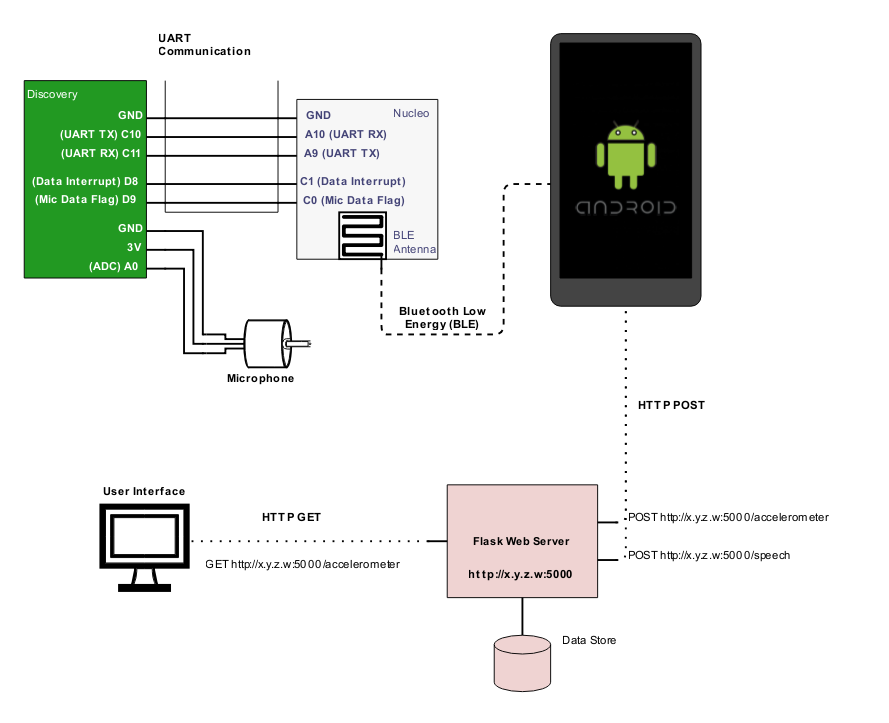
\includegraphics[scale=0.6]{systemarchitecture}
	\end{center}
\end{figure}
The Android application discussed in this paper automatically connects to the Nucleo Board when the
``\textsc{Scan for Nucleo}" button is pressed. Then, the app should receive the GATT services and
characteristics broadcast by the Nucleo, allowing for BLE communication to proceed.\\\\
With the Android app configured to send to the appropriate IP address where the Flask web server is
hosted (that is, at \texttt{http://x.y.z.w:5000} in the example in \hyperref[fig:arch]{Figure \ref{fig:arch}}),
it will automatically send the data it receives over BLE to the right endpoint of the web server. In
the event that the Android app communicates microphone data, it will then wait for an HTTP response
for the web server containing the perceived digit recognized from the audio samples, and the
response will be sent backward through the pipeline until it eventually reaches the Discovery
Board.\\\\
Upon receiving an \texttt{HTTP POST} at the \texttt{/accelerometer} endpoint, the web server will
parse the accelerometer data from the body of the request, save the data in a CSV file on the
server, and generate a graph of the data. Then, when the user interface is requested via
\texttt{HTTP GET}, the graph and the CSV data are presented on a web page.\\\\
Upon receiving an \texttt{HTTP POST} at the \texttt{/speech} endpoint, the web server will extract
the WAV file from the request and use Google Cloud's Speech API to decipher a digit from the audio
file. The digit that it perceives is then sent back to the sender of the audio data via an HTTP
response.\\\\
When the digit response containing some integer $n$ finds its way back to the Discovery board, the
Discovery's blue LED blinks $n$ times. At this stage, the process starts over, where the Discovery
waits for user input.\\\\
The remainder of this section discusses the implementation and functionality of all parts of the
system in more detail.

\subsection{The Beginning of the Pipeline: Handling the STM32 Discovery Board}
The STM32F407 Discovery Board is the microcontroller that the user interacts with. As discussed
previously, this board is responsible for gathering accelerometer and microphone data to send
through the pipeline. \hyperref[fig:discoveryfsm]{Figure \ref{fig:discoveryfsm}} demonstrates the
Finite State Machine that the Discovery Board adheres to.\\\\
\tikzstyle{decision} = [diamond, draw, fill=blue!20, text badly centered, text width=2cm, node
distance=3cm]
\tikzstyle{block} = [rectangle, draw, fill=blue!20, text centered, rounded corners, minimum
height=4em, text width=3cm, node distance=5cm]
\tikzstyle{goal} = [rectangle, draw, fill=yellow!20, text centered, rounded corners, minimum
height=4em, text width=3cm, node distance=5cm]
\tikzstyle{line} = [draw, -latex']
\tikzstyle{cloud} = [draw, ellipse, fill=red!20, node distance=7cm, text centered, text width=2cm]
\tikzstyle{label} = [draw, rectangle, text centered, text width = 3cm]
\begin{figure}[h]
	\caption{FSM on the Discovery Board}\label{fig:discoveryfsm}
	\begin{center}
		\begin{tikzpicture}[node distance = 2cm, auto, scale=0.65, transform shape]
			\node [block] (idle) {Idle};
			\node [block, draw=none, fill=none, above of=idle, node distance=2cm] (start) {Start};
			\node [block, below of=idle, node distance=3cm] (firsttap) {First Tap};
			\node [block, left of=firsttap, node distance=6cm] (singletap) {Single Tap};
			\node [block, right of=firsttap, node distance=6cm] (doubletap) {Double Tap};
			\node [block, below of=doubletap,fill=gray!20, node distance=2cm] (pause1) {One second pause};
			\node [block, below of=singletap,fill=gray!20, node distance=2cm] (pause2) {One second pause};
			\node [cloud, below of=pause1, node distance=3cm, text width=2.1cm] (acc) {Reading
			Accelerometer for 10s};
			\node [cloud, right of=acc, node distance=4cm, text width=2.5cm] (uartacc) {Transmit
			data to Nucleo over UART};
			\node [cloud, below of=pause2, node distance=3cm, text width=2.1cm] (mic) {Recording
			Microphone for 1s};
			\node [cloud, below of=mic, node distance=4cm, text width=2.5cm] (uartmic) {Transmit
			data to Nucleo over UART};
			\node [cloud, left of=uartmic, node distance=7.5cm] (response) {Blink LED $n$ times};
			\path [line] (start) -- (idle);
			\path [line] (idle) -- node {Detected tap} (firsttap);
			\path [line] (firsttap) -- node {Timed out} (singletap);
			\path [line] (firsttap) -- node {Detected tap} (doubletap);
			\path [line] (singletap) -- (pause2);
			\path [line] (doubletap) -- (pause1);
			\path [line] (pause2) -- (mic);
			\path [line] (pause1) -- (acc);
			\path [line] (mic) -- (uartmic);
			\path [line] (acc) -- (uartacc);
			\draw [->] (uartacc) to [out=90, in=0] (idle);
			\draw [->] (uartmic) to [out=0, in=330, loop] node {Waiting for response} (uartmic);
			\path [line] (uartmic) -- node {Received response $n$} (response);
			\draw [->] (response) to [out=90, in=180] (idle);
		\end{tikzpicture}
	\end{center}
\end{figure}
The system starts in the Idle state, where it waits for user input in the form of taps on the board
itself. The taps are detected by accelerometer readings polled at 100Hz over 500ms intervals, when
an accelerometer reading on the $z$ axis surpasses the average reading over the window by a certain
threshold. In order to filter out noisy accelerometer readings, an exponential moving average filter
is applied, which filters as follows:
\begin{equation}
	\hat{z}_{t} = \alpha z_{t} + (1-\alpha)\hat{z}_{t-1}, \alpha\in(0,1]
\end{equation}
where $z_t$ is the $t$th accelerometer reading, and $\hat{z}$ is $t$th output of the filter. The
parameter $\alpha$ was chosen through testing, and it represents how ``smooth" the filter output
should be.\\\\
When a tap is detected, the system enters the First Tap state, and the green LED is illuminated for
visual feedback, so the user can gauge how rapidly to make a double tap. If no tap tap is detected
in the next 500ms window, the system enters the Single Tap state (denoting that it has detected only
a single tap) and the blue LED is illuminated, and otherwise, it enters the Double Tap state where
the orange LED is illuminated. These states ultimately determine
which data to record, and how the rest of the system proceeds. In either case, there is a one second
delay after the transition to these states to allow the user to prepare for the recording.
\subsubsection{Sending Microphone Data}
In the event that the system enters the Single Tap state, after the aforementioned one second grace
period, the machine will begin to record data from the microphone. This data is sampled at 10kHz by
the onboard analog to digital converter (ADC) for 1 second using direct memory access (DMA). During
this recording period, the Discovery Board's red LED will be blinking. When the blinking stops, the
recording has finished. In
order to retain high audio quality, the ADC converts samples to 12-bit integers. Since
the FSM is not in use during the recording period, it begins to wait on a signal before continuing.
This effectively prohibits the FSM from being scheduled by the CPU until the signal is set. Once
the DMA buffer is filled with ADC readings, a callback function is triggered, which in turn sets the
signal allowing the FSM to resume.\\\\
After receiving the signal from the ADC DMA callback, the FSM can once again be scheduled. However,
before sending the microphone data to the Nucleo board, it is desired to \textit{compress} the data
returned by the DMA process. Since DMA buffers contain 32-bit words and ADC samples are only 12 bits
wide, it is desirable to \textit{squash} the data in the DMA buffer into 16-bit integers. This was
done by an elegant \texttt{squash} function, that performs this operation in place. This function can be seen in \autoref{fig:squash}. This halves the
amount of bytes required to be sent to the Nucleo board over UART.\\\\

\begin{figure}[h]
\begin{lstlisting}[
	language=C,
	basicstyle=\ttfamily\small,
	xleftmargin={0.2cm},
	tabsize=1,
]
/** Squashes an uint32_t array down to uint16_t in-place. */
void squash(uint32_t array[], int length){
	// Create two pointers, pointing at the start of the array.
	uint32_t * source = &array[0];
	uint16_t * destination = (uint16_t*) &array[0];
	for (int i=0; i<length; i++, source++, destination++){
		// We copy from source -> destination, within array.
		*destination = (uint16_t) *source;
	}
}
\end{lstlisting}
\caption{\label{fig:squash}Neat little \textit{squash()} function.}
\end{figure}







With the compressed data ready, the Discovery Board asserts a \texttt{Data Interrupt} GPIO pin,
which is directly connected to the Nucleo Board. This will trigger an interrupt on the Nucleo,
essentially informing it that it should be ready to receive a UART transmission. Furthermore, it
asserts a \texttt{Mic Data} GPIO pin, also connected directly to the Nucleo Board, which tells the
Nucleo that it is about to receive microphone data. Then, the Discovery
board begins transmitting the microphone data over UART.\\\\
Once the UART transmission is complete, the Discovery Board must wait from a response indicating how
many times its LED should blink as indicated by the microphone reading. Since the amount of time
necessary to receive the response is relatively enormous, it is undesirable for the Discovery Board
to poll for UART responses. Thus, it initiates a UART Receive in Interrupt Mode, which will trigger
an interrupt when the desired byte is received from the Nucleo Board. Meanwhile, the FSM waits on
another signal in order to prevent it from being scheduled by the CPU. This signal is set when the
UART Receive callback is triggered.\\\\
Upon receiving a response from the Nucleo Board, the discovery extracts a number
$n\in\{0,1,\dots,9\}$ from its receive buffer. Then, the blue LED will blink $n$ times, indicated
the number that was recognized from the initial microphone reading. After the LED has finished
blinking, the system returns to the Idle state, ready to start all over again. At this stage, no
LED's should be illuminated.
\subsubsection{Sending Accelerometer Data}
In the event that the system enters the Double Tap state, after the aforementioned one second grace
period, the machine will begin to record accelerometer readings at 100Hz for 10 seconds. As in the
case of the microphone recording session, the red LED will blink for the duration of the
accelerometer recording. In order to reduce the
amount of data that will be sent over UART (and later, over BLE), the Discovery Board converts each
accelerometer reading $(x_i,y_i,z_i)$ into pairs $(p_i,r_i)$, where $p_i$ and $r_i$ are the
corresponding pitch and roll measurements, respectively. Then, rather than sending $3*1000=3000$
floating point numbers, only $2*1000=2000$ floats must be sent.\\\\
Note that in contrast to the case of the microphone data, where it was desired to compress the
readings into 16-bit integers, the accelerometer data should be kept at pairs of 32-bit floats to
retain enough precision. However, before transmitting the data it is passed through an exponential
moving average filter. However, this filter uses a less smooth $\alpha$ parameter as that which was
used for detecting taps -- this is due to the fact that it was easier to detect taps when the
accelerometer readings were smoothed out as much as possible. To keep the integrity of the
accelerometer readings, less filtering was done for the recorded data.\\\\
Once the Discovery Board has finished filtering all 10000 pairs, it is ready to transmit the data
over UART to the Nucleo Board. As in the case with microphone data, the \texttt{Data Interrupt} pin
is asserted. However, in this scenario, the \texttt{Mic Data} GPIO pin is reset -- this way, the
Nucleo knows that it is about to receive accelerometer data. Next, the pitch and roll are sent in
consecutive UART transmissions. The Discovery first transmits the buffer of pitch data, and waits
10ms before transmitting the roll data. The 10ms delay allows time for the Nucleo Board to prepare
for another UART reception.\\\\
After transmitting the accelerometer data, it will eventually be uploaded to the Web Server
implemented for this project. However, in the case of accelerometer data transmission, the Discovery
Board \textit{does not} get a response. Thus, it returns immediately to the Idle state, where the
system is ready to start all over again. At this point, no LED's should be illuminated.

\subsection{The Nucleo Board}

\tikzset{
    %Define standard arrow tip
    >=stealth',
    %Define style for boxes
    punkt/.style={
           rectangle,
           rounded corners,
           draw=black, very thick,
           text width=6.5em,
           minimum height=2em,
           text centered},
    % Define arrow style
    pil/.style={
           ->,
           thick,
           shorten <=2pt,
           shorten >=2pt,}
}
\begin{tikzpicture}[node distance=5cm,on grid,auto] 
 \node[punkt] (discovery) {Discovery Board};
 \node[punkt, color=blue, right=of discovery] (nucleo) {Nucleo Board};
 \node[punkt, right=of nucleo] (phone) {Phone \\ Android};
 \node[punkt, right=of phone] (server) {Flask Server};
   \path[<->] 
   		(discovery) edge[below] node {UART} 	(nucleo)
        (nucleo) 	edge[below] node {BLE} 		(phone)
        (phone) 	edge[below] node {HTTP} 	(server)
    ;
\end{tikzpicture}

The Nucleo board acts as an intermediate between the Discovery board and the Phone. Its main role is to relay information between these two devices, using the appropriate communication protocols, and by correctly serializing and de-serializing data.

\subsubsection{UART Communication with the Discovery Board}
As described previously, the sampled data is sent over UART after each data collection period. In order to differentiate between accelerometer and microphone samples, a GPIO pin (with the alias \verb|IS_MIC_DATA|) is used. When set, the data received via UART represents microphone samples, and vice versa for accelerometer samples. Additionally, another GPIO pin, \verb|DATA_INTERRUPT|, was configured in rising-edge triggered interrupt mode, and was used to coordinate data transfers between the Discovery and Nucleo boards.

The GPIO Interrupt-Service-Routine, when triggered from the \verb|DATA_INTERRUPT| GPIO pin, sets a conditional flag, which is then read inside the main loop of the program body, and allows one execution of the \verb|pipeline()| function before being reset. This \verb|pipeline()| function contains the main logic of the Nucleo program. Its logic is fairly straightforward, and can be viewed in the diagram of \autoref{fig:nucleo_pipeline}.

\begin{figure}[h]
\centering

\tikzstyle{decision} = [diamond, draw, text badly centered, text width=2.5cm, node
distance=3cm]
\tikzstyle{block} = [rectangle, draw, text centered, rounded corners, minimum
height=4em, text width=4cm, node distance=4cm]
\tikzstyle{goal} = [rectangle, draw, fill=yellow!20, text centered, rounded corners, minimum
height=4em, text width=3cm, node distance=3cm]

\begin{tikzpicture}[shorten >=1pt,node distance=3cm,on grid,auto] 
   \node[block, initial] (wait)  {$Wait for Interrupt$}; 
   \node[decision] (mic_data)	[below=4cm of wait]	{\verb|IS_MIC_DATA|};
   \node[block] (send_acc)	[left=5cm of mic_data]	{Send Acc. Batch}; 
   \node[block] (send_mic)	[right=5cm of mic_data]	{Send Mic. Batch};
   \node[block] (wait_1) 	[below=of send_acc] {wait 10 ms};
   \node[block] (wait_2) 	[below=of send_mic] {wait 10 ms};
   \path[->]
   		(wait) edge [loop above] node {flag==0} ()
   		(wait) edge node {flag==1} (mic_data)
   		(mic_data) edge node {} (send_mic)
   		(mic_data) edge node {} (send_acc)
   		(send_mic) edge[bend left] node {$sent < 100$} (wait_2)
   		(send_mic) edge[above right, bend right] node {$sent==100$} (wait)
   		(send_acc) edge[left, bend right] node {$sent<500$} (wait_1)
   		(wait_1) edge[bend right] node {} (send_acc)
   		(send_acc) edge[bend left] node {$sent==500$} (wait)
   		(wait_2) edge[bend left] node {} (send_mic)
   ;
\end{tikzpicture}
\caption{Conceptual State-Diagram of the Nucleo board's \texttt{pipeline()} function.}
\label{fig:nucleo_pipeline}
\end{figure}

\subsubsection{Bluetooth Low Energy Communication with Phone}

In order to reliably transmit data over BLE, we have to be mindful of the throughput limitations associated with this protocol. Following some quick research, it was determined that the maximum application data that could be transmitted for a given attribute was 20 bytes\cite{blethroughput}. Given this constraint, we devised a serialization scheme for both accelerometer and microphone samples. In the case of accelerometer data, the 1000 samples of pitch and roll are interleaved, and then split into groups of two. This effectively creates packets containing
%
%\begin{figure}[h]
%\begin{tikzpicture}
%    [%%%%%%%%%%%%%%%%%%%%%%%%%%%%%%
%        box/.style={rectangle,draw=black, ultra thick, minimum size=1cm},
%    ]%%%%%%%%%%%%%%%%%%%%%%%%%%%%%%
%
%\node[box]
%
%%%pitch
%%\foreach \x/\y in {0/$p_1$, 1/$p_1$,2/$p_3$,3/$p_4$,4/(...),5/$p_1000$}
%%	\node[box] at (\x,3){\y+3};
%
%
%\foreach \x/\y in {0/$p_1$, 1/$r_1$,2/$p_2$,3/$r_2$,4/-,5/8,6/7,7/4,8/21,9/2,10/6,11/11}
%        \node[box] at (\x+3,0){\y};
%
%\draw[decorate,decoration={brace,mirror},thick] (-.5,-.7) -- node[below]{abc} (3.5,-.7);
%\draw[decorate,decoration={brace,mirror},thick] (3.5,-.7) -- node[below]{def} (7.5,-.7);
%\draw[->,very thick] (3,1.2) --  node[above,yshift=2mm]{i} (3,.7);
%\draw[->,very thick] (7,1.2) --  node[above,yshift=2mm]{j} (7,.7);
%
%\end{tikzpicture}
%\end{figure} 


%%Written by Matthew, April 20
\subsection{Smart Phone Android Application}

Given that the Nucleo board has no WiFi/Internet capabilities, data must be communicated over BLE to an Android application, that then forwards the data to the web server over HTTP. For convention, this report may use "Android app" to signify the smart phone BLE mobile application. The report also assumes that the reader has basic knowledge of telecommunication protocols, and Android applications. This portion of the report details the implementation and the rationale behind the design of the smart phone application that acts as the intermediary component between the Nucleo board and the web server.\\
With that being said, the requirements for the Android application are the following:

\begin{itemize}
    \item Scan for and connect to BLE peripheral devices;
    \item Enable the user the ability to start, or stop scanning for devices, and connect or disconnect from one peripheral device;
    \item Discover BLE services and characteristics from the peripheral device;
    \item Read voice and accelerometer data batches over BLE from the Nucleo board;
    \item Save the received data to its appropriate file;
    \item Once the accelerometer file contains 10 seconds worth of data, transmit the file to the web server over HTTP;
    \item Once the voice file contains 1 second worth of data, transmit the file to the web server over HTTP;
    \item Handle HTTP responses from the web server and send data to the Nucleo board.
\end{itemize}

Each of the Android application's business-logic features are implemented in the Java programming language, and the user interface is designed in XML. The implementation of the Android application is facilitated by using the Android Studio IDE.\\

\subsubsection{Brief Summary of Android}

The report doesn't go into detail about the code written for the project, if the reader desires to see the source code themselves, they can see it \href{https://github.com/lebrice/MicroP/tree/master/project}{here}. There is documentation written within the code so that the reader may understand the basics of the code written. This report goes into detail about the high level designs and concepts used.\\

Android applications perform in a way such that all user interface and business-logic is performed within an \textit{Activity}. Even if a developer doesn't need a user interface for their application, a main activity must instantiate and start once the user opens the application. Android developers must also declare any build dependencies such as programming libraries and hardware capabilities (such as Bluetooth and Internets) within the \textit{manifest.xml} file. The activity, since there can be multiple activities, which runs on application start up is also declared in the manifest file.\\

\subsubsection{BLE Interface}

With regards to BLE, the smart phone is recognized as the \textit{client device}, and the Nucleo board as the \textit{server device}.\\ 

The first step for any BLE handshaking, is the \textit{Scanning Phase}, which is facilitated by a \textit{BLE Scan Callback}. For the client device to recognize BLE servers, the server must advertise itself and the client must scan for these advertisements. With the push of a \textit{SCAN} button on the Android app user interface, the application enters a scanning mode which, by the help of a \textit{Scan Callback} Java class, saves scanning results as MAC addresses that the Android application could try to connect to. Since scanning is cumbersome on the smart phone's battery, the scanning automatically stops after 10 seconds to save battery life. To facilitate full automation, the Android app automatically stops scanning once it finds the Nucleo board's MAC address and tries to connect to the board. This improves the time required to enable a connection between the client and server since the user doesn't have to look through a list of MAC addresses to find the Nucleo board's address and have to select that specific address.\\

The last phase for the BLE handsaking is the connection phase, which is facilitated by a \textit{GATT Client Callback}, where GATT stands for \textit{General Attribute}. Once the Android app finds the Nucleo board, it automatically tries to connect to it, the GATT Client Callback takes charge of this operation. On the press of a CONNECT toggle button, the user can decide to connect or disconnect from the selected peripheral device.\\

The GATT Client Callback handles any connection events, and outputs statuses such as \textit{Connection Success} and \textit{Connection Failure}. Since there isn't any authentication procedure between client and server devices, the GATT Client Callback simply notifies the server that it wishes to connect to it and once the server, by the help of a GATT Server Callback, receives the notification, and responds with a connection success. If somehow the connection is a failure, the Android application simply logs the result to the Android Studio debug console. Although, on a connection success, the Android application now starts to search for \textit{Services} that the server may be transmitting. If the service used to package voice and accelerometer data is discovered, and contains their appropriate \textit{Characteristics}, the Android application is ready to read and be notified by any updates to the voice and accelerometer data.\\

At this point, the smart phone is connected to the Nucleo board over a BLE session and can now start to transmit data to one another! Exciting, if I do say so myself.

\subsubsection{Handling Data}

The Android app receives data in a byte array which is packaged under a characteristic assigned for either voice or accelerometer data. The batch of data is then written to its appropriate file with the help of the \texttt{AppController.java} class.\\

To send files over HTTP, the Android app makes use of the \href{https://developer.android.com/training/volley/index.html}{Volley Library} to create and configure HTTP requests, while also handling any HTTP responses. This is useful if the developers wish to send files conveniently over HTTP as well as receive data from the web server over HTTP. The developers wished to keep data uploading simple. By encoding the file-to-be-sent into a base-64 string and adding the encoding to the HTTP request's form, the web server can easily retrieve the file from the request by reading and decoding the form body.\\

If the web server reads the voice data file, then the Android application receives a response containing the output from the Google Speech API, under the parameter ''reading''. This contains the number that the Google Speech API was able to identify given the voice data. The Android application sends this data to the Nucleo board over BLE by writing the value to its appropriate Characteristic. At this point, the data is now handled by the Nucleo server.

\subsubsection{Summary of Project, Structure and Classes}

One can see a visualization of the Android app project structure in
\hyperref[fig:androidstructure]{Figure \ref{fig:androidstructure}}. Of course there are many files related to the application that couldn't be referenced under this report due to sizing constraints, any three dots represents that.\\

\usetikzlibrary{trees}
\tikzstyle{every node}=[draw=black,thick,anchor=west,inner sep=2pt,minimum size=1pt]
\tikzstyle{selected}=[draw=cyan,fill=cyan!30]
\begin{figure}[h]
	\caption{Overview of the Android File Hierarchy}\label{fig:androidstructure}
	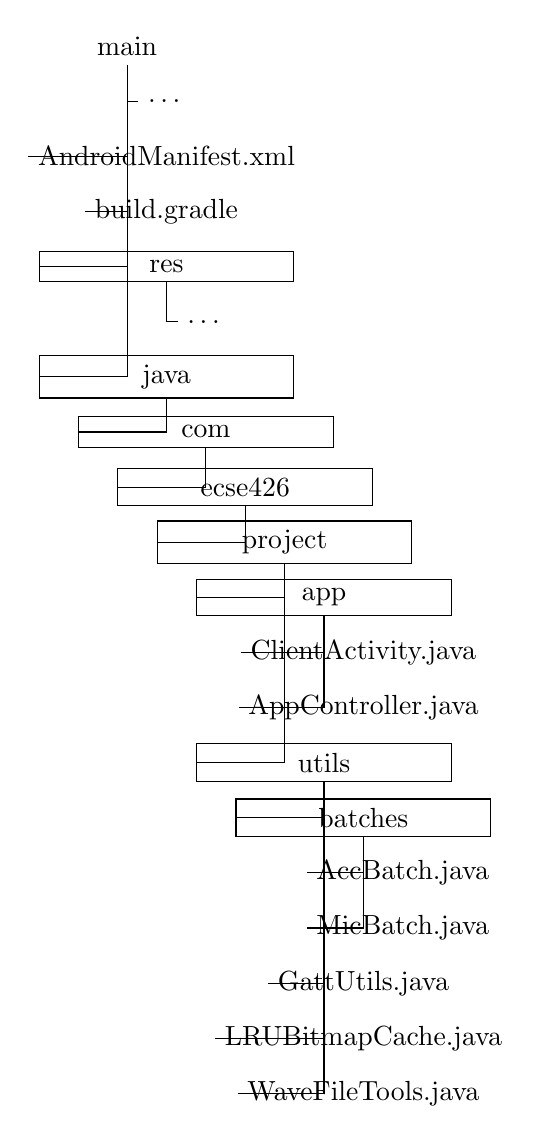
\begin{tikzpicture}[
	  grow via three points={one child at (0.5,-0.7) and
	  two children at (0.5,-0.7) and (0.5,-1.4)},   
	  edge from parent path={(\tikzparentnode.south) |- (\tikzchildnode.west)}]
	  \node {main}
		child { node [draw=none] {\ldots}}
		child { node [draw=none] {AndroidManifest.xml} }
		child { node [draw=none] {build.gradle} }
		child { node [label={[xshift=6.0cm, yshift=-0.58cm, color=gray]}] {res}
			child { node [draw=none] {\ldots}}
		}
		child [missing] {}
		child { node [label={[xshift=6.0cm, yshift=-0.58cm, color=gray]}] {java}
			child { node [label={[xshift=6.0cm, yshift=-0.58cm, color=gray]}] {com}
				child { node [label={[xshift=6.0cm, yshift=-0.58cm, color=gray]}] {ecse426}
					child { node [label={[xshift=6.0cm, yshift=-0.58cm, color=gray]}] {project}
						child { node [label={[xshift=6.0cm, yshift=-0.58cm, color=gray]}] {app}
							child { node [draw=none] {ClientActivity.java} }
							child { node [draw=none] {AppController.java} }
						}
						child [missing] {}
						child [missing] {}
						child { node [label={[xshift=6.0cm, yshift=-0.58cm, color=gray]}] {utils}
							child { node [label={[xshift=6.0cm, yshift=-0.58cm, color=gray]}] {batches}
							   child { node [draw=none] {AccBatch.java} } 
							   child { node [draw=none] {MicBatch.java} }
							}
							child [missing] {}
							child [missing] {}
							child { node [draw=none] {GattUtils.java} }
							child { node [draw=none] {LRUBitmapCache.java} }
							child { node [draw=none] {WaveFileTools.java} }
						}
					}
				}
			}
		};
	\end{tikzpicture}
\end{figure}
\tikzstyle{every node}=[] % resets borders of tables
\tikzstyle{selected}=[] % resets selected
The \texttt{AndroidManifest.xml} is the manifest file specific to this application which contains dependencies. The \texttt{build.gradle} file is the gradle build script, Android Studio automatically runs its build configurations whenever the developer runs or builds the application.\\

The \texttt{ClientActivity.java} class is the main activity that runs on start up. It is the core of the application, every other class is written around it and is used to help it. This class contains the BLE Scan Callback and GATT Client Callback logic implemented under inner classes. It handles user input and contains function calls from other classes that receive and save data over BLE and HTTP.\\

The \texttt{AppController.java} handles HTTP requests by facilitating the Client Activity with a queue for requests. It also handles reading and writing voice and accelerometer data to their appropriate files. It is important to note that the \texttt{AppController.java} class extends the Application class, making it able to run simultaneously with the \texttt{ClientActivity.java} class and have data persist when the application is closed.\\

The \texttt{AccBatch.java} and \texttt{MicBatch.java} classes are helper classes that contain functions to convert accelerometer or voice data respectively from bytes to a data type instructed by the function. The \texttt{GattUtils.java} class contains GATT Service, Characteristic, and Configuration UUIDs, as well as the Nucleo board's MAC address. The \texttt{WaveFileTools.java} class handles reading and writing data from and to files of Wave format. The \texttt{LRUBitmapCache.java} class is supposed to send and receive files, unfortunately it is not used.\\

Under the \texttt{res} directory, one can find all the user interface layouts and images. Any user interface design or image is found under that directory. 
\subsection{The End of the Pipeline: A Convenient Web Server}
In order to perform more complex data processing and to have somewhere convenient to store the
recorded data, the web server was implemented. This was achieved with the use of Python's Flask
library for creating a minimal HTTP server with a REST API and a nice, simple interface to visualize
the data that it receives.\\\\
The server has two main API endpoints, one for each of accelerometer and microphone data. Thus, if
the server is running on \texttt{151.155.209.95:48080}, the accelerometer endpoint is accessed via a
\texttt{POST} request to \texttt{151.155.209.95:48080/accelerometer}, and the microphone endpoint is
accessed via a \texttt{POST} request to \texttt{151.155.209.95:48080/speech}.\\\\
Flask manages API endpoints with a \texttt{Resource} interface. This interface provides
\texttt{get()}, \texttt{post()}, and \texttt{put()} methods, which are called when the endpoint
receives the corresponding HTTP packet. Thus, in the design of the web server, the
\texttt{Accelerometer} and \texttt{Speech} classes were created that inherit from the
\texttt{Resource} class.
\subsubsection{The Accelerometer Endpoint}
The \texttt{/accelerometer} endpoint accepts \texttt{POST} requests and is responsible for
preprocessing accelerometer data, storing the data on the server, and plotting a graph of the data
it receives. \texttt{POST} requests to this endpoint should have JSON bodies as described in
\hyperref[tab:accjson]{Table \ref{tab:accjson}}.
\begin{table}[h]
	\caption{JSON format for \texttt{POST} requests to the \texttt{/accelerometer}
	endpoint}\label{tab:accjson}
	\begin{center}
		\begin{tabular}{|c|c|c|}
			\hline
			\textbf{Parameter Name} & \textbf{Parameter Type} & \textbf{Description}\\\hline
			``accelerometer" & \texttt{[float]} & \shortstack[c]{List of accelerometer readings.\\Pitch values at
			even indices.} \\\hline
			``starttime" & \texttt{String} & \shortstack{String indicating the time\\at which the
			recordings were sent to the API.}\\\hline
		\end{tabular}
	\end{center}
\end{table}
The API system is configured bind the \texttt{Accelerometer Resource} to the \texttt{/accelerometer}
endpoint. As such, this \texttt{Resource} implements the \texttt{post()} method to handle the
accelerometer data that it is sent via \texttt{HTTP POST}.\\\\
Since the ``accelerometer" member of the \texttt{POST} request accepts an array of interleaved pitch and
roll values, the data needs to be processed such that the pitch and roll could be stored in a more
convenient format for plotting. The first task of this method is to parse the ``accelerometer"
member of the \texttt{POST} request to split up the pitch and roll data into their own respective
lists. During this procedure, the data is written to the \texttt{data.csv} file on the server in
comma-separated value (CSV) format. Each row of the CSV file contains a pitch reading and the
corresponding roll reading. Furthermore, the ``starttime" member of the \texttt{POST} is extracted
and stored in a global variable so it can later be inscribed on the user interface.\\\\
With the pitch and roll values split into their own lists, they can be graphed with relative ease.
The powerful Matplotlib\cite{matplotlib} library is used to plot the graph, and the pitch and roll
data are both plotted in the same plane. The plot is saved to the \texttt{static/graph.png} file,
and is then available to be rendered on the user interface.\\\\
Since the accelerometer communication is a one-way procedure, the \texttt{Accelerometer Resource}
has nothing interesting to return to the device that sent the \texttt{POST} request. Thus, its
response contains only an acknowledgement string.
\subsubsection{The Speech Endpoint}
Similarly to the accelerometer endpoint, implementation of the speech functionality on the web
server required the construction of a \texttt{Speech Resource}, which was bound to the
\texttt{/speech} endpoint. The files portion of the body of the \texttt{POST} requests that this
endpoint expects is shown in \hyperref[tab:micjson]{Table \ref{tab:micjson}}.\\\\
\begin{table}[h]
	\caption{Format for \texttt{POST} request files sent to the \texttt{/speech}
	endpoint}\label{tab:micjson}
	\begin{center}
		\begin{tabular}{|c|c|c|}
			\hline
			\textbf{Parameter Name} & \textbf{Parameter Type} & \textbf{Description}\\\hline
			``audio" & WAV File & \shortstack[c]{File containing audio recording in WAV format.} \\\hline
		\end{tabular}
	\end{center}
\end{table}
With the WAV file extracted from the \texttt{POST} request, the task of the speech endpoint is to
perform speech recognition. This is accomplished with the help of Google Cloud's Speech API.
Fortunately, Google Cloud provides a Python interface for their fabulous speech recognition
algorithms. The API's \texttt{transcribe\_audio()} method is called on the WAV file, and a string is
produced, containing the transcription of the audio recording. We try to cast this transcription to
an integer, and if that fails we deduce that no number could be understood from the audio recording.
In this scenario, we report a value of 0 in the \texttt{result} variable. Otherwise, \texttt{result}
is assigned the number yielded by casting the transcription to \texttt{int}.\\\\
Contrarily to the case of the accelerometer endpoint, the microphone data communication process in
this system is actually bidirectional. Thus, the sender of the microphone data expects a response
from the web server, which will be passed all the way back to the Discovery board. The
\texttt{Speech Resource}'s \texttt{post()} method returns a JSON object, which is illustrated in
\hyperref[tab:responsejson]{Table \ref{tab:responsejson}}.
\begin{table}[h]
	\caption{JSON format for the response returned by the speech endpoint to \texttt{POST}
	requests}\label{tab:responsejson}
	\begin{center}
		\begin{tabular}{|c|c|c|}
			\hline
			\textbf{Parameter Name} & \textbf{Parameter Type} & \textbf{Description}\\\hline
			``reading" & \texttt{int} & \shortstack{Byte containing the number transcribed from
			the\\input audio file. If no number is detected, 0 is returned}.\\\hline
		\end{tabular}
	\end{center}
\end{table}

\subsubsection{User Interface}
A user interface was implemented in order to have a convenient way of visualizing the accelerometer
data. This was designed as a web page hosted by the Flask server described above. To realize this
web page, a simple HTML layout was created that exploits Flask's \textit{template} functionality.
Templates allow developers to dynamically pass parameters to HTML files -- in this scenario, this
was used to dynamically update the accelerometer data and recording time shown on the page.\\\\
To access the web page, whilst assuming the web server is running on \texttt{151.155.209.95:48080},
one would navigate to \texttt{151.155.209.95:48080/accelerometer} in their favorite web browser. The
interface then displays the graph of the pitch and roll data, and shows the time at which the data
was sent directly underneath the graph. Furthermore, the UI presents a scrolling table of the CSV
data saved in \texttt{data.csv} for the user to peruse comfortably. A screenshot of this user
interface is shown in \hyperref[fig:uiscreenshot]{Figure \ref{fig:uiscreenshot}}.\\\\
\begin{figure}[h]
	\caption{Screenshot of the web server's User Interface}\label{fig:uiscreenshot}
	\begin{center}
		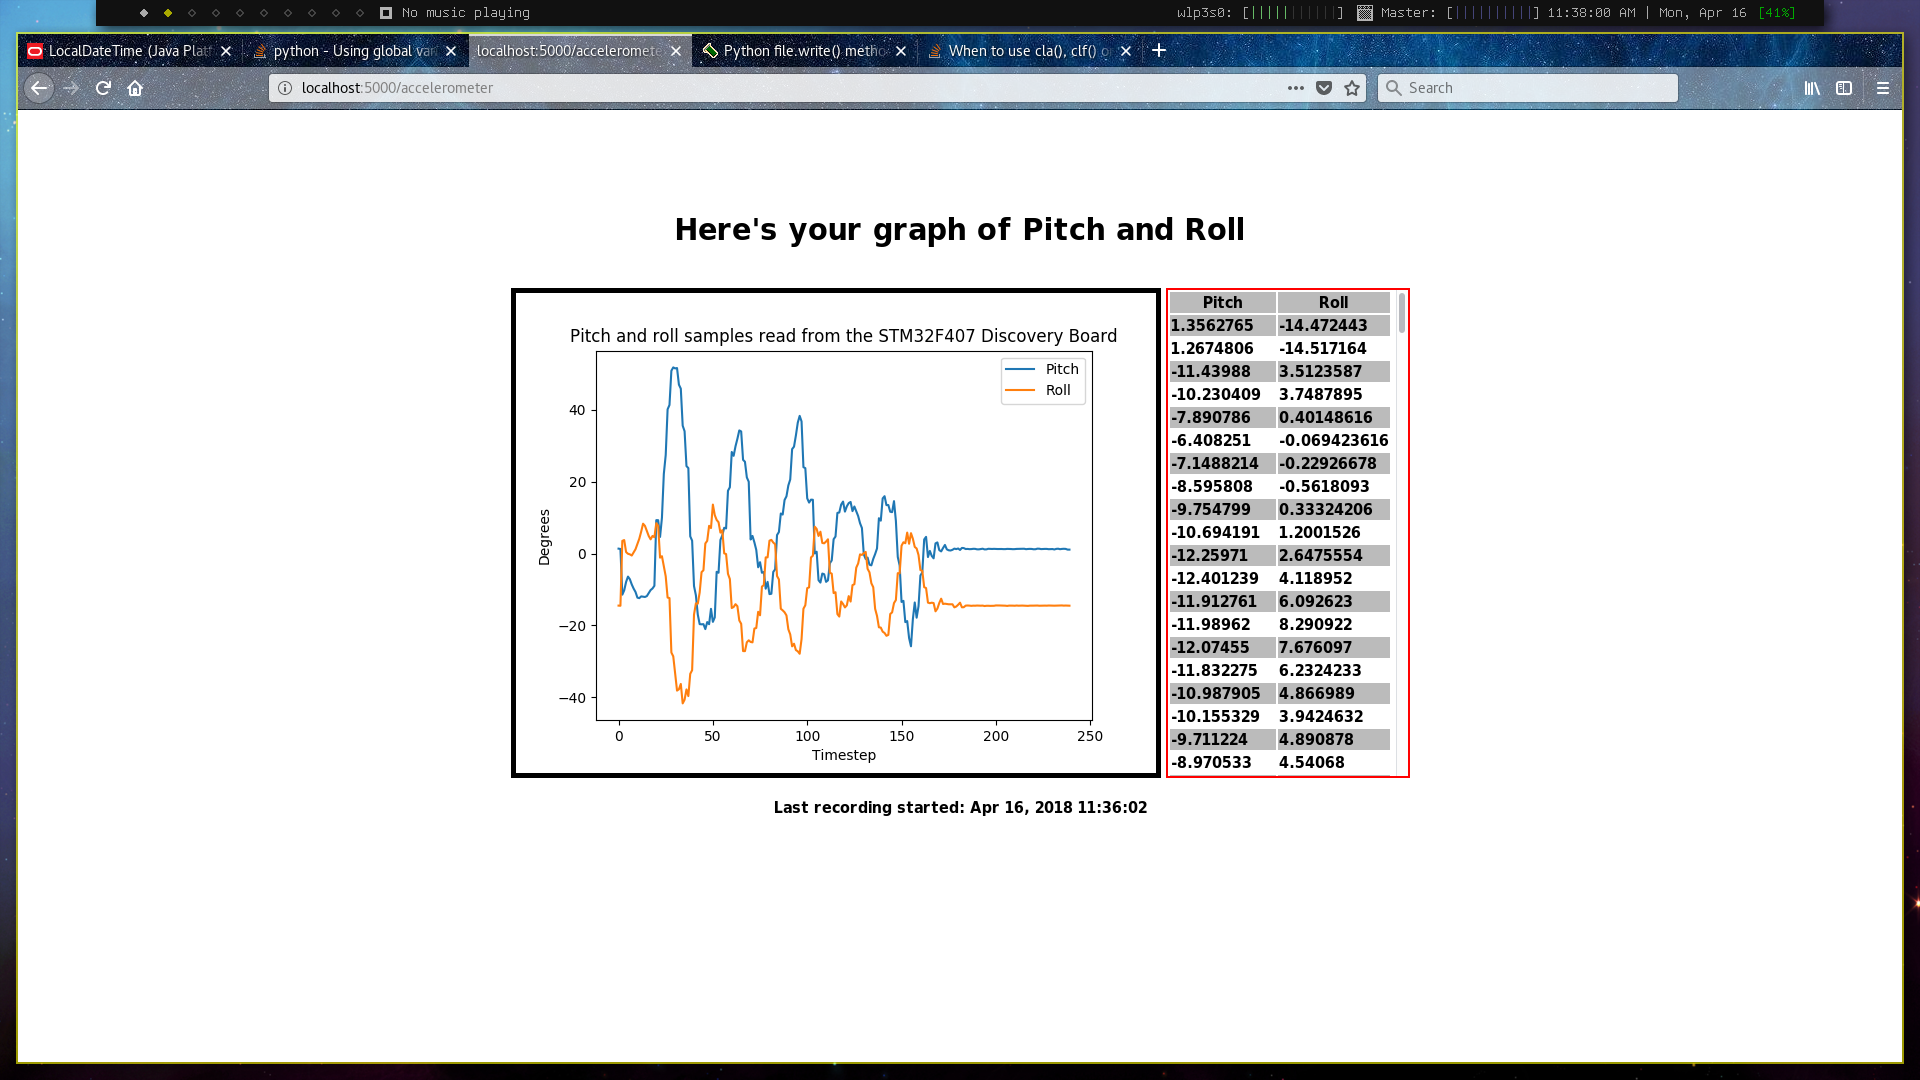
\includegraphics[width=\textwidth]{uiscreenshot}
	\end{center}
\end{figure}
In order to view the latest data, one must just refresh the web page. The graph displayed on the
user interface as well as the data used to generate the graph and the table shown are persisted on
the server, so they can be viewed offline as well.
